\begin{Exercise}[label={websec-cors-practs}]
	In this excercise we will see a practic demo of the CORS mechanism in action. To do so, we have adapted the website test-cors.org in order to simplify the excercise and be able to run it locally. 
	
	This test has two parts. The client is a simple page that serves a static page containing js code that can make diverse requests and runs on \url{localhost:8001}. The server is a NodeJS Express Server with CORS enabled and runs on \url{localhost:8000}. To run this demo, you have to run both the cors-server and cors-client. Then open a browser and go to \url{http://localhost:8001/} and open the browser developer tools (F12)
	
%{figure}[htb]
\vspace{0.2cm}
    \begin{centering}
      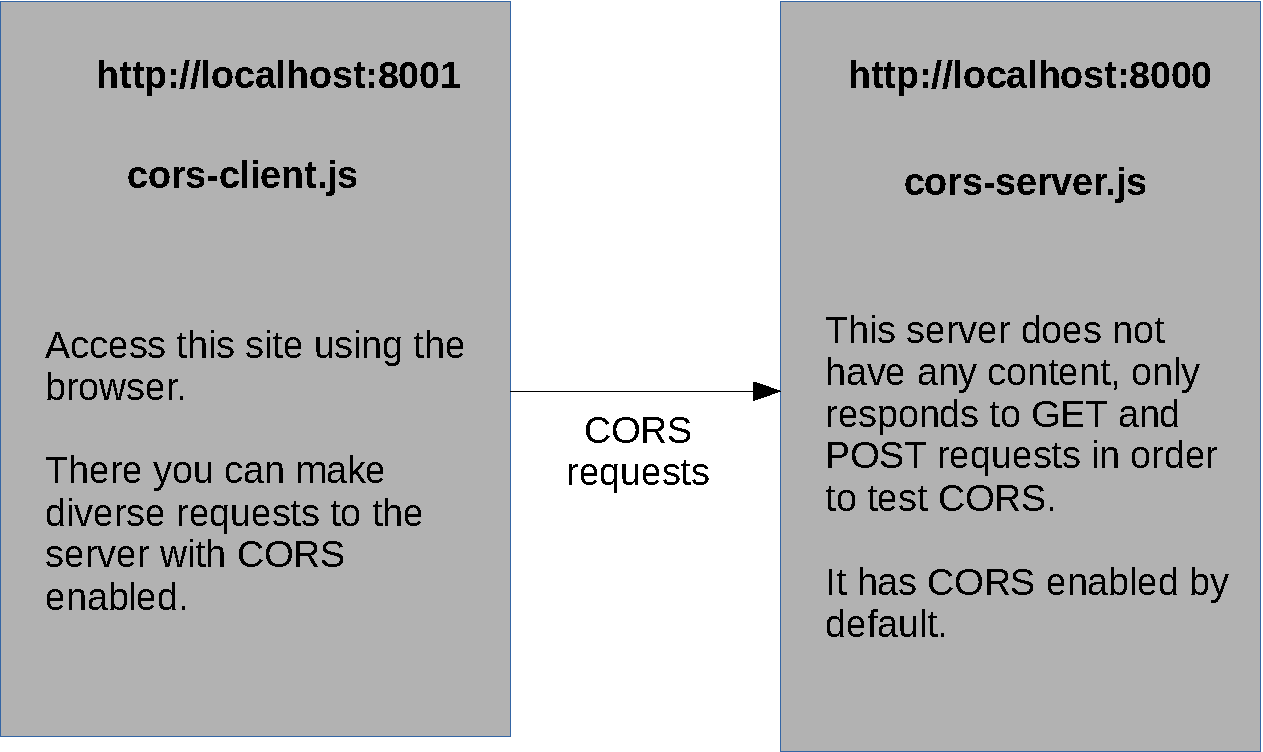
\includegraphics[width=0.7\columnwidth]{\securitydir/WebSec/figures/cors-ex}
      \par\end{centering}
%    \caption{\label{fig:cors-exc} Diagram of a CORS GET request.}
 %\end{figure}
  
	From this site you can choose which type of request you want to make, and observe a CORS request with and without pre-flight request. 
	You can also comment this line in the \textbf{cors-server.js} file to test what happens when CORS is not enabled.
	\begin{js}app.use(cors());\end{js}
  
  \subsubsection{Code}
  \begin{js}
//code-server.js
const express = require('express');
var cors = require('cors');
const app = express();

app.use(cors());

app.get('/', function (req, res) {
  res.send("ok")
});
app.put('/', function (req, res) {
  res.send("ok")
});

app.listen(8000, () => console.log('Example app listening on port 8000!'));
\end{js}

\begin{js}
 //cors-client.js
const express = require('express');
var path = require('path');
const app = express();
app.use(express.static('.'));

app.get('/', (req, res) => res.sendFile(path.join(__dirname + '/corsclient.html')));

app.listen(8001, () => console.log('Example app listening on port 8001!'));
\end{js}

\begin{html}
<!-- corsclient.html -->
<!DOCTYPE html>
<html lang="en">
<head>
<title>CORS example</title>
<link href="css/bootstrap-2.3.1.min.css" rel="stylesheet" media="screen">
</head>
<body>

<div class="container">

<div class="row">
<div class="span1"></div>
<div class="span10">
<h1>CORS example</h1>
<div class="row" id="intro">
<div class="span10">
<p>This website is a simplified version of 
<ahref="https://github.com/monsur/test-cors.org">
https://github.com/monsur/test-cors.org</a>
designed to be used locally.
All requests will be made to http://localhost:800. To view the requests made, please activate
the developer tools by pressing F12 and going to the network label.
</p>
</div>
</div>

<div class="row" id="inputs">
<div class="span10">
<form class="form-horizontal">
<legend>Client</legend>

<div class="control-group" id="client_method_div" title="Help: HTTP Method"
data-content="Which HTTP method the client should use when making the request.">
<label class="control-label" for="client_method">HTTP Method</label>
<div class="controls">
<select id="client_method" class="span2">
<option value="GET" selected>GET</option>
<option value="PUT">PUT</option>
</select>
</div>
</div>


<div class="control-group">
<div class="controls">
<button class="btn btn-large btn-primary" type="button" id="btnSendRequest">Send
Request
</button>
</div>
</div>

</form>
</div>
</div>
</div>
<div class="span1"></div>
</div>
</div>

<script src="js/jquery-1.9.1.min.js"></script>
<script src="js/bootstrap-2.3.1.min.js"></script>
<script src="js/corsclient.js"></script>

</body>
</html>
\end{html}
\end{Exercise}
